%%%%%%%%%%%%%%%%%%%%%%%%%%%%%%%%%%%%%%%%%%%%%%%%%%%%%%%%%%%%%%%%%%%%%%
% CS624: Analysis of Algorithms
% Copyright 2015 Pejman Ghorbanzade <mail@ghorbanzade.com>
% Creative Commons Attribution-ShareAlike 4.0 International License
% More info: https://bitbucket.org/ghorbanzade/umb-cs624-2015s
%%%%%%%%%%%%%%%%%%%%%%%%%%%%%%%%%%%%%%%%%%%%%%%%%%%%%%%%%%%%%%%%%%%%%%

\section*{Question 5}

Determine the cost and structure of an optimal binary search tree for a set of $n = 7$ keys with the following probabilities.

\begin{table}[H]\centering
\begin{tabular}{c|c c c c c c c c}
$i$ & 0 & 1 & 2 & 3 & 4 & 5 & 6 & 7\\
\hline
$p_i$ &      & 0.04 & 0.06 & 0.08 & 0.02 & 0.10 & 0.12 & 0.14\\
$q_i$ & 0.06 & 0.06 & 0.06 & 0.06 & 0.05 & 0.05 & 0.05 & 0.05\\
\end{tabular}
\caption{Probabilities for searching for different nodes}\label{tab51}
\end{table}

\subsection*{Solution}

To obtain the expected cost and the form of the optimal binary search tree based on the probabilities given in Table \ref{tab51}, $w(i,j)$ is calculated based on Equation \ref{eq51}.

\begin{equation}\label{eq51}
\begin{aligned}
w(i,j) &= \sum_{l = i}^{j} p_l + \sum_{l = i-1}^{j} q_l\\
&= w(i, j-1) + p_j + q_j
\end{aligned}
\end{equation}

Table \ref{tab52} provides $w(i,j)$ for all $0 \leq j \leq 7$ and $1 \leq i \leq 8$.

\begin{table}[H]\centering
\begin{tabular}{c c c c c c c c c}
  & 0    & 1    & 2    & 3    & 4    & 5    & 6    & 7\\\hline
1 & 0.06 & 0.16 & 0.28 & 0.42 & 0.49 & 0.64 & 0.81 & 1.00\\
2 &      & 0.06 & 0.18 & 0.32 & 0.39 & 0.54 & 0.71 & 0.90\\
3 &      &      & 0.06 & 0.20 & 0.27 & 0.42 & 0.59 & 0.78\\
4 &      &      &      & 0.06 & 0.13 & 0.28 & 0.45 & 0.64\\
5 &      &      &      &      & 0.05 & 0.20 & 0.37 & 0.56\\
6 &      &      &      &      &      & 0.05 & 0.22 & 0.41\\
7 &      &      &      &      &      &      & 0.05 & 0.24\\
8 &      &      &      &      &      &      &      & 0.05\\\hline
\end{tabular}
\caption{$w(i,j)$ for $0 \leq j \leq 7$ and $1 \leq i \leq 8$}\label{tab52}
\end{table}

We now calculate expected search cost $e[i,j]$ for $0 \leq j \leq 7$ and $1 \leq i \leq 8$.
We know that $e[i,j] = q_{i-1}$ when $j = i - 1$.
For the general case however where $i \leq j$, Equation \ref{eq52} can be used.

\begin{equation}\label{eq52}
\begin{aligned}
e[i,j] = \min_{i \leq r \leq j} \{e[i, r-1] + e[r+1, j] + w(i,j)\}
\end{aligned}
\end{equation}

where $r$ is the root in the optimal subtree $n_i$ to $n_j$.
Using this equation and following the \textsc{Optimal-BST} algorithm described in the textbook, $e[i, j]$ and $root[i,j]$ are obtained as shown in Table \ref{tab53} and Table \ref{tab54}, respectively.

\begin{table}[H]\centering
\begin{tabular}{c c c c c c c c c}
  & 0    & 1    & 2    & 3    & 4    & 5    & 6    & 7\\\hline
1 & 0.06 & 0.28 & 0.50 & 0.76 & 0.90 & 1.18 & 1.50 & 1.86\\
2 &      & 0.06 & 0.30 & 0.56 & 0.70 & 0.98 & 1.30 & 1.66\\
3 &      &      & 0.06 & 0.32 & 0.46 & 0.74 & 1.06 & 1.42\\
4 &      &      &      & 0.06 & 0.30 & 0.46 & 0.78 & 1.14\\
5 &      &      &      &      & 0.05 & 0.24 & 0.62 & 0.98\\
6 &      &      &      &      &      & 0.05 & 0.32 & 0.68\\
7 &      &      &      &      &      &      & 0.05 & 0.34\\
8 &      &      &      &      &      &      &      & 0.05\\\hline
\end{tabular}
\caption{$e[i,j]$ for $0 \leq j \leq 7$ and $1 \leq i \leq 8$}\label{tab53}
\end{table}

\begin{table}[H]\centering
\begin{tabular}{c c c c c c c c c}
  & 1    & 2    & 3 & 4 & 5 & 6 & 7\\\hline
1 & 1 & 2 & 3 & 3 & 5 & 6 & 7\\
2 &   & 2 & 3 & 3 & 5 & 6 & 7\\
3 &   &   & 3 & 3 & 5 & 6 & 7\\
4 &   &   &   & 4 & 5 & 6 & 7\\
5 &   &   &   &   & 5 & 6 & 7\\
6 &   &   &   &   &   & 6 & 7\\
7 &   &   &   &   &   &   & 7\\\hline
\end{tabular}
\caption{$root[i,j]$ for $1 \leq i,j \leq 7$}\label{tab54}
\end{table}

And the binary tree can now be constructed based on Table \ref{tab54}, as shown in Figure \ref{fig51}.

\begin{figure}[H]\centering
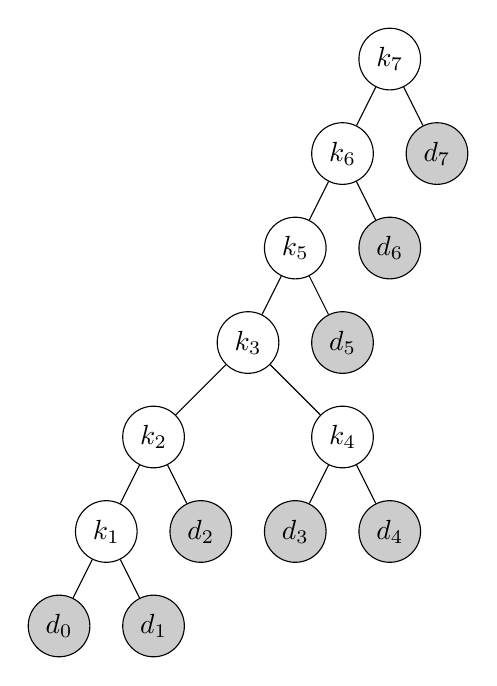
\begin{tikzpicture}[level distance=1.5cm,
  level 4/.style={sibling distance=3cm},
  level 5/.style={sibling distance=1.5cm},scale=0.8]
\node[circle,draw]{$k_7$}
child{
  node[circle,draw]{$k_6$}
  child{
    node[circle,draw]{$k_5$}
    child {
      node[circle,draw]{$k_3$}
      child {
        node[circle,draw]{$k_2$}
        child {
          node[circle,draw]{$k_1$}
          child {
            node[circle,draw,fill=black!20]{$d_0$}
          }
          child {
            node[circle,draw,fill=black!20]{$d_1$}
          }
        }
        child {
          node[circle,draw,fill=black!20]{$d_2$}
        }
      }
      child {
        node[circle,draw]{$k_4$}
        child {
          node[circle,draw,fill=black!20]{$d_3$}
        }
        child {
          node[circle,draw,fill=black!20]{$d_4$}
        }
      }
    }
    child {
      node[circle,draw,fill=black!20]{$d_5$}
    }
  }
  child{
    node[circle,draw,fill=black!20]{$d_6$}
  }
}
child{
  node[circle,draw,fill=black!20]{$d_7$}
};
\end{tikzpicture}
\caption{Optimal binary search tree based on given probabilities}\label{fig51}
\end{figure}

The total cost of the tree can also be easily computed using Table \ref{tab55} given below.

\begin{table}[H]\centering
\begin{tabular}{c c c c | c c c c}
node & depth & probability & contribution & node & depth & probability & contribution\\\hline
$k_1$ & 5 & 0.04 & 0.24 & $d_0$ & 6 & 0.06 & 0.42\\
$k_2$ & 4 & 0.06 & 0.30 & $d_1$ & 6 & 0.06 & 0.42\\
$k_3$ & 3 & 0.08 & 0.32 & $d_2$ & 5 & 0.06 & 0.36\\
$k_4$ & 4 & 0.02 & 0.10 & $d_3$ & 5 & 0.06 & 0.36\\
$k_5$ & 2 & 0.10 & 0.30 & $d_4$ & 5 & 0.05 & 0.30\\
$k_6$ & 1 & 0.12 & 0.24 & $d_5$ & 3 & 0.05 & 0.20\\
$k_7$ & 0 & 0.14 & 0.14 & $d_6$ & 2 & 0.05 & 0.15\\
      &   &      &      & $d_7$ & 1 & 0.05 & 0.10\\\hline
\end{tabular}
\caption{$root[i,j]$ for $1 \leq i,j \leq 7$}\label{tab55}
\end{table}

By summing over the contribution of each node, the entire cost of this binary search tree is found to be 3.95.
